\documentclass[../main.tex]{subfiles}

\begin{document}
	
In order to objectively evaluate the performance of our inference algorithms, we simulate the price and returns of a tradable commodity using the 2 dimensional discrete time state space model described in \autoref{eq:2__2__1__drift_corrected_simple_PF}. This provides us with the ground truth state that we can use to compare with the inferred state estimates from our particle filter.

This also allows us to check that the model has the appropriate characteristics that we are looking for. 

\begin{figure}[h!]
	\centering
	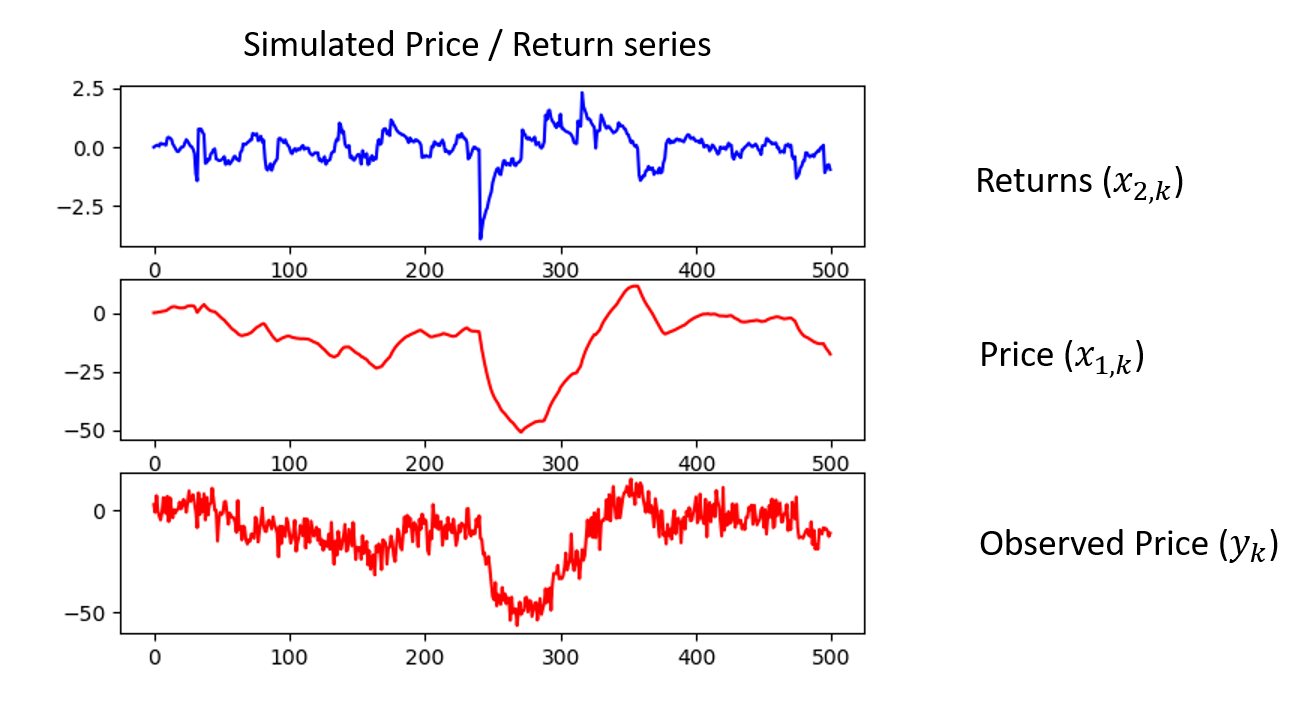
\includegraphics[width=12.0cm]{../plots/3__1__1__simulation.png}
	\caption{Simulation Results for 500 iterations}
	\label{fig:3__1__1__simulation}
\end{figure}


Figure \ref{fig:3__1__1__simulation} shows a simulated price($x_1$) / returns($x_2$) series, together with the observed price series corrupted by gaussian noise($y$). 

We note that the returns series has the desired jump activity, together with a gaussian drift back to zero mean. The gaussian drift back to zero mean allows for a predictable trend to be captured in the price process, while the jump activity allows for sharp changes in the trend. 

This shows that the state-space model described in \autoref{eq:2__2__1__drift_corrected_simple_PF} is able to capture both a predictable trend in asset prices, as well as sharp changes in these trends, both extremely useful for a momentum-based strategy. 

\end{document}

